% 原分章PDF第50页7.1.5.4标题至第54页7.2标题前。
\subsubsection{离散数据因果推断的加性噪声模型}
本节介绍加性噪声模型方法（Shimizu et al. 2006；Peters et al. 2011），用于从离散数据中发现因果方向$X\to Y$或$Y\to X$。离散数据的加性噪声因果推断可应用于复杂疾病的全基因组因果研究；这类研究考察疾病变量与SNP基因型变量这两个离散变量之间的因果关系。

\bookdeepheading{paragraph}{7.1.5.4.1}{整数模型}
先考虑整数加性噪声模型：
\begin{equation}
Y=f(X)+N_1,\qquad N_1\perp X,\tag{7.192}
\end{equation}
其中$X$、$Y$是两个整数随机变量，$f:Z\to Z$将整数空间中的值映射到整数空间，$N_1$为取整数值且独立于假定原因$X$的加性噪声。式(7.192)称为从$X$到$Y$的正向加性噪声模型。还可以定义从$Y$到$X$的反向加性噪声模型：
\begin{equation}
X=g(Y)+N_2,\qquad N_2\perp Y,\tag{7.193}
\end{equation}
其中$g:Z\to Z$将整数空间中的值映射到整数空间，$N_2$为取整数值且独立于假定原因$Y$的加性噪声。

正向和反向的两个加性噪声模型能否同时很好地拟合数据？这是利用加性噪声模型判断因果方向的基本问题。考虑一个平凡例子：$P(X=0)=1$、$f(0)=0$、$P(N_1=0)=1$、$P(Y=0)=1$、$g(0)=0$、$P(N_2=0)=1$。显然，这些分布同时满足两个方向的加性噪声模型(7.192)与(7.193)。不过，这种情形非常少见（Peters et al. 2011）。在大多数情况下，正向或反向的加性疾病模型之一能够拟合数据，但两个模型不能同时拟合数据。若两个模型都能拟合数据，就无法选择因果方向。图7.4中的联合分布只允许从$X$到$Y$的加性噪声模型（ANM），不允许从$Y$到$X$的模型；而图7.5中的联合分布允许从$X$到$Y$、从$Y$到$X$两个方向的ANM。

\begin{figure}[htbp]
\centering
% 原PDF矢量路径与精确点位转为可编辑TikZ；未模拟点位。
\definecolor{chSevenADPlot4C0}{rgb}{0.136690,0.121950,0.125292}
\definecolor{chSevenADPlot4C1}{rgb}{0.218204,0.367498,0.543938}
\definecolor{chSevenADPlot4C2}{rgb}{0.305257,0.508278,0.748669}
\resizebox{.74\linewidth}{!}{
\begin{tikzpicture}[x=1bp,y=-1bp,line cap=round,line join=round]
\path[use as bounding box] (0,0) rectangle (270.00000,175.00000);
\path[line width=0.5000bp,draw=chSevenADPlot4C0,fill=none] (10.27900,152.38397) --(236.22699,152.38397);
\path[line width=0.5000bp,draw=chSevenADPlot4C0,fill=none] (233.18301,150.62299) --(236.22699,152.38397) --(233.18301,154.14496);
\path[line width=0.5000bp,draw=chSevenADPlot4C0,fill=none] (28.96900,168.27100) --(28.96900,10.39600);
\path[line width=0.5000bp,draw=chSevenADPlot4C0,fill=none] (30.74500,13.41498) --(28.97000,10.39600) --(27.19300,13.41498);
\path[line width=0.5000bp,draw=chSevenADPlot4C1,fill=chSevenADPlot4C2] (58.35300,132.53796) .. controls (58.35300,131.80701) and (59.54800,131.21399) .. (61.02299,131.21399) .. controls (62.49699,131.21399) and (63.69299,131.80701) .. (63.69299,132.53796) .. controls (63.69299,133.26996) and (62.49699,133.86200) .. (61.02299,133.86200) .. controls (59.54800,133.86200) and (58.35300,133.26996) .. (58.35300,132.53796) --cycle;
\path[line width=0.5000bp,draw=chSevenADPlot4C1,fill=chSevenADPlot4C2] (74.37300,137.54297) .. controls (74.37300,136.81201) and (75.56799,136.21802) .. (77.04300,136.21802) .. controls (78.51801,136.21802) and (79.71300,136.81201) .. (79.71300,137.54297) .. controls (79.71300,138.27399) and (78.51801,138.86597) .. (77.04300,138.86597) .. controls (75.56799,138.86597) and (74.37300,138.27399) .. (74.37300,137.54297) --cycle;
\path[line width=0.5000bp,draw=chSevenADPlot4C1,fill=chSevenADPlot4C2] (90.39301,139.05200) .. controls (90.39301,138.32001) and (91.58800,137.72797) .. (93.06300,137.72797) .. controls (94.53799,137.72797) and (95.73300,138.32001) .. (95.73300,139.05200) .. controls (95.73300,139.78296) and (94.53799,140.37598) .. (93.06300,140.37598) .. controls (91.58800,140.37598) and (90.39301,139.78296) .. (90.39301,139.05200) --cycle;
\path[line width=0.5000bp,draw=chSevenADPlot4C1,fill=chSevenADPlot4C2] (106.41400,139.31702) .. controls (106.41400,138.58496) and (107.60800,137.99298) .. (109.08299,137.99298) .. controls (110.55701,137.99298) and (111.75301,138.58496) .. (111.75301,139.31702) .. controls (111.75301,140.04797) and (110.55701,140.64099) .. (109.08299,140.64099) .. controls (107.60800,140.64099) and (106.41400,140.04797) .. (106.41400,139.31702) --cycle;
\path[line width=0.5000bp,draw=chSevenADPlot4C1,fill=chSevenADPlot4C2] (122.21899,137.14600) .. controls (122.21899,136.41400) and (123.41499,135.82196) .. (124.88901,135.82196) .. controls (126.36501,135.82196) and (127.55901,136.41400) .. (127.55901,137.14600) .. controls (127.55901,137.87695) and (126.36501,138.46997) .. (124.88901,138.46997) .. controls (123.41499,138.46997) and (122.21899,137.87695) .. (122.21899,137.14600) --cycle;
\path[line width=0.5000bp,draw=chSevenADPlot4C1,fill=chSevenADPlot4C2] (140.75000,132.67096) .. controls (140.75000,131.93896) and (141.94501,131.34698) .. (143.42000,131.34698) .. controls (144.89400,131.34698) and (146.09000,131.93896) .. (146.09000,132.67096) .. controls (146.09000,133.40198) and (144.89400,133.99500) .. (143.42000,133.99500) .. controls (141.94501,133.99500) and (140.75000,133.40198) .. (140.75000,132.67096) --cycle;
\path[line width=0.5000bp,draw=chSevenADPlot4C1,fill=chSevenADPlot4C2] (157.46400,120.67700) .. controls (157.46400,119.94501) and (158.66000,119.35297) .. (160.13300,119.35297) .. controls (161.60800,119.35297) and (162.80399,119.94501) .. (162.80399,120.67700) .. controls (162.80399,121.40796) and (161.60800,122.00000) .. (160.13300,122.00000) .. controls (158.66000,122.00000) and (157.46400,121.40796) .. (157.46400,120.67700) --cycle;
\path[line width=0.5000bp,draw=chSevenADPlot4C1,fill=chSevenADPlot4C2] (170.20001,119.53796) .. controls (170.20001,118.80701) and (171.39499,118.21399) .. (172.87000,118.21399) .. controls (174.34399,118.21399) and (175.54001,118.80701) .. (175.54001,119.53796) .. controls (175.54001,120.26996) and (174.34399,120.86200) .. (172.87000,120.86200) .. controls (171.39499,120.86200) and (170.20001,120.26996) .. (170.20001,119.53796) --cycle;
\path[line width=0.5000bp,draw=chSevenADPlot4C1,fill=chSevenADPlot4C2] (183.89700,119.98798) .. controls (183.89700,119.25696) and (185.09201,118.66400) .. (186.56799,118.66400) .. controls (188.04199,118.66400) and (189.23801,119.25696) .. (189.23801,119.98798) .. controls (189.23801,120.71899) and (188.04199,121.31097) .. (186.56799,121.31097) .. controls (185.09201,121.31097) and (183.89700,120.71899) .. (183.89700,119.98798) --cycle;
\path[line width=0.5000bp,draw=chSevenADPlot4C1,fill=chSevenADPlot4C2] (198.98199,119.98798) .. controls (198.98199,119.25696) and (200.17801,118.66400) .. (201.65302,118.66400) .. controls (203.12900,118.66400) and (204.32300,119.25696) .. (204.32300,119.98798) .. controls (204.32300,120.71899) and (203.12900,121.31097) .. (201.65302,121.31097) .. controls (200.17801,121.31097) and (198.98199,120.71899) .. (198.98199,119.98798) --cycle;
\path[line width=0.5000bp,draw=chSevenADPlot4C1,fill=chSevenADPlot4C2] (213.21500,119.35297) .. controls (213.21500,118.62201) and (214.41000,118.02795) .. (215.88400,118.02795) .. controls (217.35800,118.02795) and (218.55399,118.62201) .. (218.55399,119.35297) .. controls (218.55399,120.08398) and (217.35800,120.67700) .. (215.88400,120.67700) .. controls (214.41000,120.67700) and (213.21500,120.08398) .. (213.21500,119.35297) --cycle;
\path[line width=0.5000bp,draw=chSevenADPlot4C1,fill=chSevenADPlot4C2] (58.35300,121.86700) .. controls (58.35300,121.13696) and (59.54800,120.54401) .. (61.02299,120.54401) .. controls (62.49699,120.54401) and (63.69299,121.13696) .. (63.69299,121.86700) .. controls (63.69299,122.59998) and (62.49699,123.19098) .. (61.02299,123.19098) .. controls (59.54800,123.19098) and (58.35300,122.59998) .. (58.35300,121.86700) --cycle;
\path[line width=0.5000bp,draw=chSevenADPlot4C1,fill=chSevenADPlot4C2] (74.45300,125.83899) .. controls (74.45300,125.10797) and (75.64799,124.51501) .. (77.12300,124.51501) .. controls (78.59801,124.51501) and (79.79300,125.10797) .. (79.79300,125.83899) .. controls (79.79300,126.57001) and (78.59801,127.16296) .. (77.12300,127.16296) .. controls (75.64799,127.16296) and (74.45300,126.57001) .. (74.45300,125.83899) --cycle;
\path[line width=0.5000bp,draw=chSevenADPlot4C1,fill=chSevenADPlot4C2] (90.71300,127.16296) .. controls (90.71300,126.43201) and (91.90800,125.83899) .. (93.38300,125.83899) .. controls (94.85800,125.83899) and (96.05400,126.43201) .. (96.05400,127.16296) .. controls (96.05400,127.89398) and (94.85800,128.48700) .. (93.38300,128.48700) .. controls (91.90800,128.48700) and (90.71300,127.89398) .. (90.71300,127.16296) --cycle;
\path[line width=0.5000bp,draw=chSevenADPlot4C1,fill=chSevenADPlot4C2] (106.49300,128.48700) .. controls (106.49300,127.39001) and (107.68800,126.50098) .. (109.16299,126.50098) .. controls (110.63800,126.50098) and (111.83299,127.39001) .. (111.83299,128.48700) .. controls (111.83299,129.58398) and (110.63800,130.47198) .. (109.16299,130.47198) .. controls (107.68800,130.47198) and (106.49300,129.58398) .. (106.49300,128.48700) --cycle;
\path[line width=0.5000bp,draw=chSevenADPlot4C1,fill=chSevenADPlot4C2] (121.49899,125.60095) .. controls (121.49899,124.86902) and (122.69400,124.27698) .. (124.16800,124.27698) .. controls (125.64400,124.27698) and (126.83900,124.86902) .. (126.83900,125.60095) .. controls (126.83900,126.33197) and (125.64400,126.92499) .. (124.16800,126.92499) .. controls (122.69400,126.92499) and (121.49899,126.33197) .. (121.49899,125.60095) --cycle;
\path[line width=0.5000bp,draw=chSevenADPlot4C1,fill=chSevenADPlot4C2] (138.48000,120.86200) .. controls (138.48000,120.13098) and (139.67500,119.53796) .. (141.14999,119.53796) .. controls (142.62500,119.53796) and (143.82001,120.13098) .. (143.82001,120.86200) .. controls (143.82001,121.59302) and (142.62500,122.18597) .. (141.14999,122.18597) .. controls (139.67500,122.18597) and (138.48000,121.59302) .. (138.48000,120.86200) --cycle;
\path[line width=0.5000bp,draw=chSevenADPlot4C1,fill=chSevenADPlot4C2] (156.04900,112.57397) .. controls (156.04900,111.84302) and (157.24400,111.25098) .. (158.71800,111.25098) .. controls (160.19400,111.25098) and (161.38800,111.84302) .. (161.38800,112.57397) .. controls (161.38800,113.30499) and (160.19400,113.89899) .. (158.71800,113.89899) .. controls (157.24400,113.89899) and (156.04900,113.30499) .. (156.04900,112.57397) --cycle;
\path[line width=0.5000bp,draw=chSevenADPlot4C1,fill=chSevenADPlot4C2] (169.69299,106.80096) .. controls (169.69299,106.07098) and (170.88699,105.47699) .. (172.36301,105.47699) .. controls (173.83801,105.47699) and (175.03201,106.07098) .. (175.03201,106.80096) .. controls (175.03201,107.53296) and (173.83801,108.12500) .. (172.36301,108.12500) .. controls (170.88699,108.12500) and (169.69299,107.53296) .. (169.69299,106.80096) --cycle;
\path[line width=0.5000bp,draw=chSevenADPlot4C1,fill=chSevenADPlot4C2] (183.65701,106.80096) .. controls (183.65701,106.07098) and (184.85199,105.47699) .. (186.32700,105.47699) .. controls (187.80099,105.47699) and (188.99701,106.07098) .. (188.99701,106.80096) .. controls (188.99701,107.53296) and (187.80099,108.12500) .. (186.32700,108.12500) .. controls (184.85199,108.12500) and (183.65701,107.53296) .. (183.65701,106.80096) --cycle;
\path[line width=0.5000bp,draw=chSevenADPlot4C1,fill=chSevenADPlot4C2] (199.30301,107.59497) .. controls (199.30301,106.86401) and (200.49899,106.27197) .. (201.97299,106.27197) .. controls (203.44800,106.27197) and (204.64301,106.86401) .. (204.64301,107.59497) .. controls (204.64301,108.32697) and (203.44800,108.91998) .. (201.97299,108.91998) .. controls (200.49899,108.91998) and (199.30301,108.32697) .. (199.30301,107.59497) --cycle;
\path[line width=0.5000bp,draw=chSevenADPlot4C1,fill=chSevenADPlot4C2] (213.21500,106.24500) .. controls (213.21500,105.51398) and (214.41000,104.92200) .. (215.88400,104.92200) .. controls (217.35800,104.92200) and (218.55399,105.51398) .. (218.55399,106.24500) .. controls (218.55399,106.97595) and (217.35800,107.57001) .. (215.88400,107.57001) .. controls (214.41000,107.57001) and (213.21500,106.97595) .. (213.21500,106.24500) --cycle;
\path[line width=0.5000bp,draw=chSevenADPlot4C1,fill=chSevenADPlot4C2] (58.35300,110.21802) .. controls (58.35300,109.48596) and (59.54800,108.89301) .. (61.02299,108.89301) .. controls (62.49699,108.89301) and (63.69299,109.48596) .. (63.69299,110.21802) .. controls (63.69299,110.94897) and (62.49699,111.54199) .. (61.02299,111.54199) .. controls (59.54800,111.54199) and (58.35300,110.94897) .. (58.35300,110.21802) --cycle;
\path[line width=0.5000bp,draw=chSevenADPlot4C1,fill=chSevenADPlot4C2] (74.66701,113.97797) .. controls (74.66701,113.24695) and (75.86200,112.65295) .. (77.33701,112.65295) .. controls (78.81200,112.65295) and (80.00700,113.24695) .. (80.00700,113.97797) .. controls (80.00700,114.70898) and (78.81200,115.30096) .. (77.33701,115.30096) .. controls (75.86200,115.30096) and (74.66701,114.70898) .. (74.66701,113.97797) --cycle;
\path[line width=0.5000bp,draw=chSevenADPlot4C1,fill=chSevenADPlot4C2] (90.39301,116.44000) .. controls (90.39301,115.70898) and (91.58800,115.11597) .. (93.06300,115.11597) .. controls (94.53799,115.11597) and (95.73300,115.70898) .. (95.73300,116.44000) .. controls (95.73300,117.17200) and (94.53799,117.76398) .. (93.06300,117.76398) .. controls (91.58800,117.76398) and (90.39301,117.17200) .. (90.39301,116.44000) --cycle;
\path[line width=0.5000bp,draw=chSevenADPlot4C1,fill=chSevenADPlot4C2] (106.54700,119.53796) .. controls (106.54700,118.80701) and (107.74200,118.21399) .. (109.21600,118.21399) .. controls (110.69099,118.21399) and (111.88600,118.80701) .. (111.88600,119.53796) .. controls (111.88600,120.26996) and (110.69099,120.86200) .. (109.21600,120.86200) .. controls (107.74200,120.86200) and (106.54700,120.26996) .. (106.54700,119.53796) --cycle;
\path[line width=0.5000bp,draw=chSevenADPlot4C1,fill=chSevenADPlot4C2] (122.08600,113.97797) .. controls (122.08600,113.24695) and (123.28101,112.65295) .. (124.75600,112.65295) .. controls (126.23100,112.65295) and (127.42599,113.24695) .. (127.42599,113.97797) .. controls (127.42599,114.70898) and (126.23100,115.30096) .. (124.75600,115.30096) .. controls (123.28101,115.30096) and (122.08600,114.70898) .. (122.08600,113.97797) --cycle;
\path[line width=0.5000bp,draw=chSevenADPlot4C1,fill=chSevenADPlot4C2] (136.98399,108.91998) .. controls (136.98399,108.18799) and (138.17999,107.59497) .. (139.65500,107.59497) .. controls (141.13000,107.59497) and (142.32500,108.18799) .. (142.32500,108.91998) .. controls (142.32500,109.65100) and (141.13000,110.24402) .. (139.65500,110.24402) .. controls (138.17999,110.24402) and (136.98399,109.65100) .. (136.98399,108.91998) --cycle;
\path[line width=0.5000bp,draw=chSevenADPlot4C1,fill=chSevenADPlot4C2] (154.79401,104.15399) .. controls (154.79401,103.42297) and (155.98900,102.82996) .. (157.46400,102.82996) .. controls (158.93800,102.82996) and (160.13300,103.42297) .. (160.13300,104.15399) .. controls (160.13300,104.88501) and (158.93800,105.47699) .. (157.46400,105.47699) .. controls (155.98900,105.47699) and (154.79401,104.88501) .. (154.79401,104.15399) --cycle;
\path[line width=0.5000bp,draw=chSevenADPlot4C1,fill=chSevenADPlot4C2] (169.69299,96.65997) .. controls (169.69299,95.92896) and (170.88699,95.33600) .. (172.36301,95.33600) .. controls (173.83801,95.33600) and (175.03201,95.92896) .. (175.03201,96.65997) .. controls (175.03201,97.39099) and (173.83801,97.98401) .. (172.36301,97.98401) .. controls (170.88699,97.98401) and (169.69299,97.39099) .. (169.69299,96.65997) --cycle;
\path[line width=0.5000bp,draw=chSevenADPlot4C1,fill=chSevenADPlot4C2] (184.27100,96.84595) .. controls (184.27100,96.11499) and (185.46600,95.52197) .. (186.94101,95.52197) .. controls (188.41599,95.52197) and (189.61200,96.11499) .. (189.61200,96.84595) .. controls (189.61200,97.57697) and (188.41599,98.16998) .. (186.94101,98.16998) .. controls (185.46600,98.16998) and (184.27100,97.57697) .. (184.27100,96.84595) --cycle;
\path[line width=0.5000bp,draw=chSevenADPlot4C1,fill=chSevenADPlot4C2] (198.60901,95.91901) .. controls (198.60901,95.18799) and (199.80399,94.59497) .. (201.27899,94.59497) .. controls (202.75500,94.59497) and (203.94901,95.18799) .. (203.94901,95.91901) .. controls (203.94901,96.64996) and (202.75500,97.24200) .. (201.27899,97.24200) .. controls (199.80399,97.24200) and (198.60901,96.64996) .. (198.60901,95.91901) --cycle;
\path[line width=0.5000bp,draw=chSevenADPlot4C1,fill=chSevenADPlot4C2] (186.29999,87.52496) .. controls (186.29999,86.79401) and (187.49600,86.20099) .. (188.96899,86.20099) .. controls (190.44501,86.20099) and (191.64001,86.79401) .. (191.64001,87.52496) .. controls (191.64001,88.25598) and (190.44501,88.84900) .. (188.96899,88.84900) .. controls (187.49600,88.84900) and (186.29999,88.25598) .. (186.29999,87.52496) --cycle;
\path[line width=0.5000bp,draw=chSevenADPlot4C1,fill=chSevenADPlot4C2] (58.35300,98.56702) .. controls (58.35300,97.83600) and (59.54800,97.24200) .. (61.02299,97.24200) .. controls (62.49699,97.24200) and (63.69299,97.83600) .. (63.69299,98.56702) .. controls (63.69299,99.29797) and (62.49699,99.89001) .. (61.02299,99.89001) .. controls (59.54800,99.89001) and (58.35300,99.29797) .. (58.35300,98.56702) --cycle;
\path[line width=0.5000bp,draw=chSevenADPlot4C1,fill=chSevenADPlot4C2] (74.07899,103.38501) .. controls (74.07899,102.65497) and (75.27400,102.06201) .. (76.74899,102.06201) .. controls (78.22400,102.06201) and (79.41901,102.65497) .. (79.41901,103.38501) .. controls (79.41901,104.11700) and (78.22400,104.70996) .. (76.74899,104.70996) .. controls (75.27400,104.70996) and (74.07899,104.11700) .. (74.07899,103.38501) --cycle;
\path[line width=0.5000bp,draw=chSevenADPlot4C1,fill=chSevenADPlot4C2] (90.71300,106.51001) .. controls (90.71300,105.77899) and (91.90800,105.18597) .. (93.38300,105.18597) .. controls (94.85800,105.18597) and (96.05400,105.77899) .. (96.05400,106.51001) .. controls (96.05400,107.24097) and (94.85800,107.83398) .. (93.38300,107.83398) .. controls (91.90800,107.83398) and (90.71300,107.24097) .. (90.71300,106.51001) --cycle;
\path[line width=0.5000bp,draw=chSevenADPlot4C1,fill=chSevenADPlot4C2] (106.41400,110.27002) .. controls (106.41400,109.53900) and (107.60800,108.94598) .. (109.08299,108.94598) .. controls (110.55701,108.94598) and (111.75301,109.53900) .. (111.75301,110.27002) .. controls (111.75301,111.00195) and (110.55701,111.59399) .. (109.08299,111.59399) .. controls (107.60800,111.59399) and (106.41400,111.00195) .. (106.41400,110.27002) --cycle;
\path[line width=0.5000bp,draw=chSevenADPlot4C1,fill=chSevenADPlot4C2] (121.49899,103.38501) .. controls (121.49899,102.65497) and (122.69400,102.06201) .. (124.16800,102.06201) .. controls (125.64400,102.06201) and (126.83900,102.65497) .. (126.83900,103.38501) .. controls (126.83900,104.11700) and (125.64400,104.70996) .. (124.16800,104.70996) .. controls (122.69400,104.70996) and (121.49899,104.11700) .. (121.49899,103.38501) --cycle;
\path[line width=0.5000bp,draw=chSevenADPlot4C1,fill=chSevenADPlot4C2] (134.31500,98.06396) .. controls (134.31500,97.33197) and (135.50900,96.73999) .. (136.98399,96.73999) .. controls (138.46001,96.73999) and (139.65500,97.33197) .. (139.65500,98.06396) .. controls (139.65500,98.79498) and (138.46001,99.38800) .. (136.98399,99.38800) .. controls (135.50900,99.38800) and (134.31500,98.79498) .. (134.31500,98.06396) --cycle;
\path[line width=0.5000bp,draw=chSevenADPlot4C1,fill=chSevenADPlot4C2] (153.38000,94.01196) .. controls (153.38000,93.28101) and (154.57401,92.68799) .. (156.04900,92.68799) .. controls (157.52299,92.68799) and (158.71800,93.28101) .. (158.71800,94.01196) .. controls (158.71800,94.74402) and (157.52299,95.33600) .. (156.04900,95.33600) .. controls (154.57401,95.33600) and (153.38000,94.74402) .. (153.38000,94.01196) --cycle;
\path[line width=0.5000bp,draw=chSevenADPlot4C1,fill=chSevenADPlot4C2] (213.21500,98.56702) .. controls (213.21500,97.83600) and (214.41000,97.24200) .. (215.88400,97.24200) .. controls (217.35800,97.24200) and (218.55399,97.83600) .. (218.55399,98.56702) .. controls (218.55399,99.29797) and (217.35800,99.89001) .. (215.88400,99.89001) .. controls (214.41000,99.89001) and (213.21500,99.29797) .. (213.21500,98.56702) --cycle;
\path[line width=0.5000bp,draw=chSevenADPlot4C1,fill=chSevenADPlot4C2] (169.63901,87.52496) .. controls (169.63901,86.79401) and (170.83499,86.20099) .. (172.30899,86.20099) .. controls (173.78500,86.20099) and (174.97900,86.79401) .. (174.97900,87.52496) .. controls (174.97900,88.25598) and (173.78500,88.84900) .. (172.30899,88.84900) .. controls (170.83499,88.84900) and (169.63901,88.25598) .. (169.63901,87.52496) --cycle;
\path[line width=0.5000bp,draw=chSevenADPlot4C1,fill=chSevenADPlot4C2] (198.60901,87.52496) .. controls (198.60901,86.79401) and (199.80399,86.20099) .. (201.27899,86.20099) .. controls (202.75500,86.20099) and (203.94901,86.79401) .. (203.94901,87.52496) .. controls (203.94901,88.25598) and (202.75500,88.84900) .. (201.27899,88.84900) .. controls (199.80399,88.84900) and (198.60901,88.25598) .. (198.60901,87.52496) --cycle;
\path[line width=0.5000bp,draw=chSevenADPlot4C1,fill=chSevenADPlot4C2] (212.54700,88.26599) .. controls (212.54700,87.53497) and (213.74200,86.94299) .. (215.21600,86.94299) .. controls (216.69199,86.94299) and (217.88599,87.53497) .. (217.88599,88.26599) .. controls (217.88599,88.99799) and (216.69199,89.58997) .. (215.21600,89.58997) .. controls (213.74200,89.58997) and (212.54700,88.99799) .. (212.54700,88.26599) --cycle;
\node[inner sep=0pt,font=\fontsize{8}{9}\selectfont] at (237.88150,164.69562) {$\mathrm{X}$};
\node[inner sep=0pt,font=\fontsize{8}{9}\selectfont] at (16.87592,19.06363) {$\mathrm{Y}$};
\end{tikzpicture}
}

\origfig{4}{联合分布允许$X\to Y$方向的ANM，但不允许$Y\to X$方向的ANM。}
\end{figure}

\bookdeepheading{paragraph}{7.1.5.4.2}{循环模型}
先介绍取模运算与有限环$Z/mZ$。对整数$a$和$b$作除法，写为
\[
\frac ab=k\quad\text{余数为 }r.
\]
这里关心的是余数$r$，定义$r$为$a$模$b$的余数，记作$r=a\bmod b$。例如，$14\bmod3=2$。有限环$Z/mZ$定义为按$n$取模时所有可能余数的集合，即
\[
Z/mZ=\{Z\bmod m\}=\{0,1,\ldots,m-1\}.
\]
下面定义循环加性噪声模型（Peters et al. 2011）。设$X$和$Y$分别为$m$循环与$\widetilde m$循环随机变量，$f:Z/mZ\to Z/\widetilde m Z$为一个函数，$N$为$\widetilde m$循环噪声。定义从$X$到$Y$的加性噪声模型为
\begin{equation}
Y=f(X)+N,\qquad N\perp X,\tag{7.194}
\end{equation}
其中$N$独立于$X$，且$P(N=0)>P(N=j)$，$j\ne0$。若该模型可逆，则存在函数$g:Z/\widetilde m Z\to Z/mZ$以及$m$循环噪声$\widetilde N$，使得
\begin{equation}
X=g(Y)+\widetilde N,\qquad \widetilde N\perp Y.\tag{7.195}
\end{equation}
某些例子表明，联合分布可以允许正反两个方向的ANM。不过，在一般情形下，ANM是可识别的（Peters et al. 2011）。已有研究讨论了ANM可识别性的部分条件（Peters et al. 2011），但这些条件较为复杂，限于本书篇幅，此处不再介绍。

\begin{figure}[htbp]
\centering
% 原PDF矢量路径与精确点位转为可编辑TikZ；未模拟点位。
\definecolor{chSevenADPlot5C0}{rgb}{0.136690,0.121950,0.125292}
\definecolor{chSevenADPlot5C1}{rgb}{0.286748,0.497444,0.740063}
\definecolor{chSevenADPlot5C2}{rgb}{0.218204,0.367498,0.543938}
\definecolor{chSevenADPlot5C3}{rgb}{0.305257,0.508278,0.748669}
\resizebox{.74\linewidth}{!}{
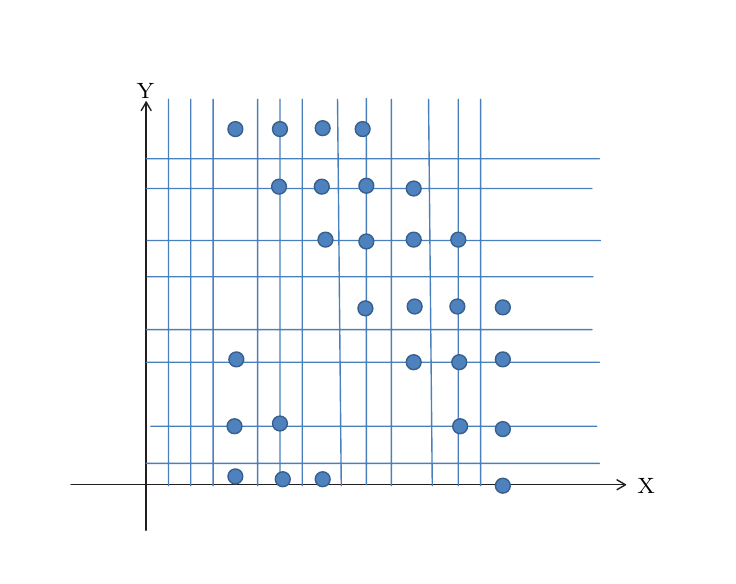
\begin{tikzpicture}[x=1bp,y=-1bp,line cap=round,line join=round]
\path[use as bounding box] (0,0) rectangle (245.00000,190.00000);
\path[line width=0.5000bp,draw=chSevenADPlot5C0,fill=none] (15.59700,164.55099) --(215.19199,164.55099);
\path[line width=0.5000bp,draw=chSevenADPlot5C0,fill=none] (212.14200,162.77197) --(215.19199,164.55099) --(212.14200,166.32898);
\path[line width=0.5000bp,draw=chSevenADPlot5C0,fill=none] (42.66499,180.92099) --(42.66499,26.79498);
\path[line width=0.5000bp,draw=chSevenADPlot5C0,fill=none] (44.44299,29.84399) --(42.66499,26.79498) --(40.88600,29.84399);
\path[line width=0.5000bp,draw=chSevenADPlot5C1,fill=none] (42.67799,120.43198) --(205.83301,120.43198) (43.02499,76.62097) --(206.17999,76.62097) (42.67799,47.20001) --(205.83301,47.20001) (58.72600,25.80298) --(58.72600,164.88498) (90.82300,25.80298) --(90.82300,164.88498) (121.92799,25.48199) --(121.92799,164.56400) (155.01401,25.80298) --(155.01401,164.88498) (42.67799,156.86099) --(205.83301,156.86099) (44.36301,143.48798) --(204.84399,143.48798) (42.67799,108.71698) --(203.15900,108.71698) (43.02499,89.67398) --(203.50601,89.67398) (42.67799,57.89899) --(203.15900,57.89899) (50.70200,25.80298) --(50.70200,164.88498) (66.75000,25.80298) --(66.75000,164.88498) (82.79800,25.80298) --(82.79800,164.88498) (98.84599,25.80298) --(98.84599,164.88498) (111.55099,25.80298) --(112.88901,164.88498) (130.94200,25.80298) --(130.94200,164.88498) (144.31599,25.80298) --(145.65300,164.88498) (163.03900,25.80298) --(163.03900,164.88498);
\path[line width=0.5000bp,draw=chSevenADPlot5C2,fill=chSevenADPlot5C3] (72.09900,36.50098) .. controls (72.09900,35.02399) and (73.29700,33.82599) .. (74.77400,33.82599) .. controls (76.25101,33.82599) and (77.44901,35.02399) .. (77.44901,36.50098) .. controls (77.44901,37.97900) and (76.25101,39.17596) .. (74.77400,39.17596) .. controls (73.29700,39.17596) and (72.09900,37.97900) .. (72.09900,36.50098) --cycle;
\path[line width=0.5000bp,draw=chSevenADPlot5C2,fill=chSevenADPlot5C3] (87.82600,57.22998) .. controls (87.82600,55.75299) and (89.02400,54.55499) .. (90.50101,54.55499) .. controls (91.97800,54.55499) and (93.17599,55.75299) .. (93.17599,57.22998) .. controls (93.17599,58.70697) and (91.97800,59.90399) .. (90.50101,59.90399) .. controls (89.02400,59.90399) and (87.82600,58.70697) .. (87.82600,57.22998) --cycle;
\path[line width=0.5000bp,draw=chSevenADPlot5C2,fill=chSevenADPlot5C3] (88.14799,36.50098) .. controls (88.14799,35.02399) and (89.34500,33.82599) .. (90.82300,33.82599) .. controls (92.30000,33.82599) and (93.49699,35.02399) .. (93.49699,36.50098) .. controls (93.49699,37.97900) and (92.30000,39.17596) .. (90.82300,39.17596) .. controls (89.34500,39.17596) and (88.14799,37.97900) .. (88.14799,36.50098) --cycle;
\path[line width=0.5000bp,draw=chSevenADPlot5C2,fill=chSevenADPlot5C3] (89.16400,162.55899) .. controls (89.16400,161.08099) and (90.36200,159.88397) .. (91.83800,159.88397) .. controls (93.31599,159.88397) and (94.51199,161.08099) .. (94.51199,162.55899) .. controls (94.51199,164.03598) and (93.31599,165.23297) .. (91.83800,165.23297) .. controls (90.36200,165.23297) and (89.16400,164.03598) .. (89.16400,162.55899) --cycle;
\path[line width=0.5000bp,draw=chSevenADPlot5C2,fill=chSevenADPlot5C3] (103.20599,57.22998) .. controls (103.20599,55.75299) and (104.40300,54.55499) .. (105.88000,54.55499) .. controls (107.35800,54.55499) and (108.55499,55.75299) .. (108.55499,57.22998) .. controls (108.55499,58.70697) and (107.35800,59.90399) .. (105.88000,59.90399) .. controls (104.40300,59.90399) and (103.20599,58.70697) .. (103.20599,57.22998) --cycle;
\path[line width=0.5000bp,draw=chSevenADPlot5C2,fill=chSevenADPlot5C3] (153.00800,143.48798) .. controls (153.00800,142.01099) and (154.20599,140.81299) .. (155.68201,140.81299) .. controls (157.16000,140.81299) and (158.35699,142.01099) .. (158.35699,143.48798) .. controls (158.35699,144.96500) and (157.16000,146.16199) .. (155.68201,146.16199) .. controls (154.20599,146.16199) and (153.00800,144.96500) .. (153.00800,143.48798) --cycle;
\path[line width=0.5000bp,draw=chSevenADPlot5C2,fill=chSevenADPlot5C3] (118.90601,101.04099) .. controls (118.90601,99.56400) and (120.10300,98.36697) .. (121.58099,98.36697) .. controls (123.05701,98.36697) and (124.25600,99.56400) .. (124.25600,101.04099) .. controls (124.25600,102.51797) and (123.05701,103.71597) .. (121.58099,103.71597) .. controls (120.10300,103.71597) and (118.90601,102.51797) .. (118.90601,101.04099) --cycle;
\path[line width=0.5000bp,draw=chSevenADPlot5C2,fill=chSevenADPlot5C3] (72.44701,119.41599) .. controls (72.44701,117.93900) and (73.64400,116.74100) .. (75.12199,116.74100) .. controls (76.59900,116.74100) and (77.79700,117.93900) .. (77.79700,119.41599) .. controls (77.79700,120.89398) and (76.59900,122.09000) .. (75.12199,122.09000) .. controls (73.64400,122.09000) and (72.44701,120.89398) .. (72.44701,119.41599) --cycle;
\path[line width=0.5000bp,draw=chSevenADPlot5C2,fill=chSevenADPlot5C3] (136.63901,100.37198) .. controls (136.63901,98.89499) and (137.83701,97.69800) .. (139.31400,97.69800) .. controls (140.79201,97.69800) and (141.98900,98.89499) .. (141.98900,100.37198) .. controls (141.98900,101.84900) and (140.79201,103.04700) .. (139.31400,103.04700) .. controls (137.83701,103.04700) and (136.63901,101.84900) .. (136.63901,100.37198) --cycle;
\path[line width=0.5000bp,draw=chSevenADPlot5C2,fill=chSevenADPlot5C3] (103.52699,162.55899) .. controls (103.52699,161.08099) and (104.72400,159.88397) .. (106.20200,159.88397) .. controls (107.67900,159.88397) and (108.87601,161.08099) .. (108.87601,162.55899) .. controls (108.87601,164.03598) and (107.67900,165.23297) .. (106.20200,165.23297) .. controls (104.72400,165.23297) and (103.52699,164.03598) .. (103.52699,162.55899) --cycle;
\path[line width=0.5000bp,draw=chSevenADPlot5C2,fill=chSevenADPlot5C3] (119.25301,56.90900) .. controls (119.25301,55.43201) and (120.45100,54.23401) .. (121.92799,54.23401) .. controls (123.40500,54.23401) and (124.60201,55.43201) .. (124.60201,56.90900) .. controls (124.60201,58.38599) and (123.40500,59.58398) .. (121.92799,59.58398) .. controls (120.45100,59.58398) and (119.25301,58.38599) .. (119.25301,56.90900) --cycle;
\path[line width=0.5000bp,draw=chSevenADPlot5C2,fill=chSevenADPlot5C3] (136.29201,57.89899) .. controls (136.29201,56.42096) and (137.48801,55.22400) .. (138.96700,55.22400) .. controls (140.44299,55.22400) and (141.64101,56.42096) .. (141.64101,57.89899) .. controls (141.64101,59.37598) and (140.44299,60.57300) .. (138.96700,60.57300) .. controls (137.48801,60.57300) and (136.29201,59.37598) .. (136.29201,57.89899) --cycle;
\path[line width=0.5000bp,draw=chSevenADPlot5C2,fill=chSevenADPlot5C3] (104.54300,76.30096) .. controls (104.54300,74.82300) and (105.74100,73.62598) .. (107.21800,73.62598) .. controls (108.69501,73.62598) and (109.89301,74.82300) .. (109.89301,76.30096) .. controls (109.89301,77.77802) and (108.69501,78.97498) .. (107.21800,78.97498) .. controls (105.74100,78.97498) and (104.54300,77.77802) .. (104.54300,76.30096) --cycle;
\path[line width=0.5000bp,draw=chSevenADPlot5C2,fill=chSevenADPlot5C3] (103.52699,36.17999) .. controls (103.52699,34.70300) and (104.72400,33.50598) .. (106.20200,33.50598) .. controls (107.67900,33.50598) and (108.87601,34.70300) .. (108.87601,36.17999) .. controls (108.87601,37.65698) and (107.67900,38.85498) .. (106.20200,38.85498) .. controls (104.72400,38.85498) and (103.52699,37.65698) .. (103.52699,36.17999) --cycle;
\path[line width=0.5000bp,draw=chSevenADPlot5C2,fill=chSevenADPlot5C3] (117.91600,36.50098) .. controls (117.91600,35.02399) and (119.11400,33.82599) .. (120.59200,33.82599) .. controls (122.06799,33.82599) and (123.26500,35.02399) .. (123.26500,36.50098) .. controls (123.26500,37.97900) and (122.06799,39.17596) .. (120.59200,39.17596) .. controls (119.11400,39.17596) and (117.91600,37.97900) .. (117.91600,36.50098) --cycle;
\path[line width=0.5000bp,draw=chSevenADPlot5C2,fill=chSevenADPlot5C3] (119.25301,76.96899) .. controls (119.25301,75.49200) and (120.45100,74.29401) .. (121.92799,74.29401) .. controls (123.40500,74.29401) and (124.60201,75.49200) .. (124.60201,76.96899) .. controls (124.60201,78.44598) and (123.40500,79.64398) .. (121.92799,79.64398) .. controls (120.45100,79.64398) and (119.25301,78.44598) .. (119.25301,76.96899) --cycle;
\path[line width=0.5000bp,draw=chSevenADPlot5C2,fill=chSevenADPlot5C3] (136.29201,76.30096) .. controls (136.29201,74.82300) and (137.48801,73.62598) .. (138.96700,73.62598) .. controls (140.44299,73.62598) and (141.64101,74.82300) .. (141.64101,76.30096) .. controls (141.64101,77.77802) and (140.44299,78.97498) .. (138.96700,78.97498) .. controls (137.48801,78.97498) and (136.29201,77.77802) .. (136.29201,76.30096) --cycle;
\path[line width=0.5000bp,draw=chSevenADPlot5C2,fill=chSevenADPlot5C3] (152.34000,76.30096) .. controls (152.34000,74.82300) and (153.53700,73.62598) .. (155.01401,73.62598) .. controls (156.49100,73.62598) and (157.68900,74.82300) .. (157.68900,76.30096) .. controls (157.68900,77.77802) and (156.49100,78.97498) .. (155.01401,78.97498) .. controls (153.53700,78.97498) and (152.34000,77.77802) .. (152.34000,76.30096) --cycle;
\path[line width=0.5000bp,draw=chSevenADPlot5C2,fill=chSevenADPlot5C3] (152.01801,100.37198) .. controls (152.01801,98.89499) and (153.21600,97.69800) .. (154.69299,97.69800) .. controls (156.17099,97.69800) and (157.36801,98.89499) .. (157.36801,100.37198) .. controls (157.36801,101.84900) and (156.17099,103.04700) .. (154.69299,103.04700) .. controls (153.21600,103.04700) and (152.01801,101.84900) .. (152.01801,100.37198) --cycle;
\path[line width=0.5000bp,draw=chSevenADPlot5C2,fill=chSevenADPlot5C3] (168.38800,100.69299) .. controls (168.38800,99.21597) and (169.58499,98.01898) .. (171.06299,98.01898) .. controls (172.54001,98.01898) and (173.73801,99.21597) .. (173.73801,100.69299) .. controls (173.73801,102.17099) and (172.54001,103.36798) .. (171.06299,103.36798) .. controls (169.58499,103.36798) and (168.38800,102.17099) .. (168.38800,100.69299) --cycle;
\path[line width=0.5000bp,draw=chSevenADPlot5C2,fill=chSevenADPlot5C3] (71.77800,143.48798) .. controls (71.77800,142.01099) and (72.97600,140.81299) .. (74.45300,140.81299) .. controls (75.92999,140.81299) and (77.12801,142.01099) .. (77.12801,143.48798) .. controls (77.12801,144.96500) and (75.92999,146.16199) .. (74.45300,146.16199) .. controls (72.97600,146.16199) and (71.77800,144.96500) .. (71.77800,143.48798) --cycle;
\path[line width=0.5000bp,draw=chSevenADPlot5C2,fill=chSevenADPlot5C3] (168.38800,164.88498) .. controls (168.38800,163.40900) and (169.58499,162.20999) .. (171.06299,162.20999) .. controls (172.54001,162.20999) and (173.73801,163.40900) .. (173.73801,164.88498) .. controls (173.73801,166.36298) and (172.54001,167.56000) .. (171.06299,167.56000) .. controls (169.58499,167.56000) and (168.38800,166.36298) .. (168.38800,164.88498) --cycle;
\path[line width=0.5000bp,draw=chSevenADPlot5C2,fill=chSevenADPlot5C3] (136.29201,120.43198) .. controls (136.29201,118.95499) and (137.48801,117.75699) .. (138.96700,117.75699) .. controls (140.44299,117.75699) and (141.64101,118.95499) .. (141.64101,120.43198) .. controls (141.64101,121.90997) and (140.44299,123.10699) .. (138.96700,123.10699) .. controls (137.48801,123.10699) and (136.29201,121.90997) .. (136.29201,120.43198) --cycle;
\path[line width=0.5000bp,draw=chSevenADPlot5C2,fill=chSevenADPlot5C3] (152.68700,120.43198) .. controls (152.68700,118.95499) and (153.88499,117.75699) .. (155.36200,117.75699) .. controls (156.84000,117.75699) and (158.03699,118.95499) .. (158.03699,120.43198) .. controls (158.03699,121.90997) and (156.84000,123.10699) .. (155.36200,123.10699) .. controls (153.88499,123.10699) and (152.68700,121.90997) .. (152.68700,120.43198) --cycle;
\path[line width=0.5000bp,draw=chSevenADPlot5C2,fill=chSevenADPlot5C3] (168.38800,119.41599) .. controls (168.38800,117.93900) and (169.58499,116.74100) .. (171.06299,116.74100) .. controls (172.54001,116.74100) and (173.73801,117.93900) .. (173.73801,119.41599) .. controls (173.73801,120.89398) and (172.54001,122.09000) .. (171.06299,122.09000) .. controls (169.58499,122.09000) and (168.38800,120.89398) .. (168.38800,119.41599) --cycle;
\path[line width=0.5000bp,draw=chSevenADPlot5C2,fill=chSevenADPlot5C3] (88.14799,142.49799) .. controls (88.14799,141.02100) and (89.34500,139.82397) .. (90.82300,139.82397) .. controls (92.30000,139.82397) and (93.49699,141.02100) .. (93.49699,142.49799) .. controls (93.49699,143.97598) and (92.30000,145.17297) .. (90.82300,145.17297) .. controls (89.34500,145.17297) and (88.14799,143.97598) .. (88.14799,142.49799) --cycle;
\path[line width=0.5000bp,draw=chSevenADPlot5C2,fill=chSevenADPlot5C3] (168.38800,144.50497) .. controls (168.38800,143.02698) and (169.58499,141.82999) .. (171.06299,141.82999) .. controls (172.54001,141.82999) and (173.73801,143.02698) .. (173.73801,144.50497) .. controls (173.73801,145.98199) and (172.54001,147.17999) .. (171.06299,147.17999) .. controls (169.58499,147.17999) and (168.38800,145.98199) .. (168.38800,144.50497) --cycle;
\path[line width=0.5000bp,draw=chSevenADPlot5C2,fill=chSevenADPlot5C3] (72.09900,161.54099) .. controls (72.09900,160.06497) and (73.29700,158.86798) .. (74.77400,158.86798) .. controls (76.25101,158.86798) and (77.44901,160.06497) .. (77.44901,161.54099) .. controls (77.44901,163.01999) and (76.25101,164.21698) .. (74.77400,164.21698) .. controls (73.29700,164.21698) and (72.09900,163.01999) .. (72.09900,161.54099) --cycle;
\node[inner sep=0pt,font=\fontsize{8}{9}\selectfont] at (222.62875,164.99533) {$\mathrm{X}$};
\node[inner sep=0pt,font=\fontsize{8}{9}\selectfont] at (42.53423,22.62335) {$\mathrm{Y}$};
\end{tikzpicture}
}

\origfig{5}{联合分布允许两个方向的ANM。}
\end{figure}

\bookdeepheading{paragraph}{7.1.5.4.3}{离散变量ANM的统计检验}
在实际应用中，利用离散变量ANM进行因果推断的关键问题，是建立相应的统计检验。Peters et al.（2011）提出了基于ANM进行因果推断的一般流程，现重述于结论7.25。

\par\medskip\Needspace{5\baselineskip}\noindent\textbf{结论7.25：利用ANM进行因果推断的一般流程}\par
利用ANM进行因果推断的一般步骤如下。
\begin{enumerate}[label=\textbf{步骤\arabic*.},leftmargin=4.8em]
\item 输入$n$个数据样本$\{(x_1,y_1),\ldots,(x_n,y_n)\}$。
\item 对正向模型$Y=f(X)+N$进行非线性回归，计算残差$\widehat N_i=y_i-f(x_i)$，$i=1,\ldots,n$。
\item 对反向模型$X=g(Y)+\widetilde N$进行非线性回归，计算残差$\widehat{\widetilde N}_i=x_i-g(y_i)$，$i=1,\ldots,n$。
\item 若残差$\widehat N$独立于$X$，而$\widetilde N$不独立于$Y$，则$X$导致$Y$（$X\to Y$）；若$\widehat N$不独立于$X$，而$\widetilde N$独立于$Y$，则$Y$导致$X$（$Y\to X$）。
\item 若$\widehat N$独立于$X$且$\widetilde N$独立于$Y$，或$\widehat N$不独立于$X$且$\widetilde N$也不独立于$Y$，则无法作出判定，此时因果关系未知。
\end{enumerate}

要实施这些流程，需要发展离散变量的非线性回归统计方法，以及检验两个随机变量独立性的统计量（Peters et al. 2011）。先介绍离散变量的回归。目标是选取回归函数，使残差尽可能独立于回归变量（潜在原因），因此，可将残差与回归变量之间的依赖性度量作为回归的损失函数。对ANM $Y=f(X)+N$，将这一度量记为$\operatorname{DM}(\widehat N,X)$。令$\widehat P(X,Y)$为联合分布$P(X,Y)$的样本分布。下面给出基于距离相关的回归，它能够涵盖多元情形，也可视为Peters et al.（2011）论文中算法1的简单推广。在结论7.26中，将单变量ANM推广到多变量ANM，并假设$W$是$m$维变量向量、$Z$是$q$维变量向量。多变量ANM写为
\[
Z=F(W)+N,
\]
其中$Z=[Z_1,\ldots,Z_m]$，$W=[W_1,\ldots,W_q]$，$F(W)=[f_1(W),\ldots,f_m(W)]$，$N=[N_1,\ldots,N_m]$，并且$N$独立于$W$。

\par\medskip\Needspace{5\baselineskip}\noindent\textbf{结论7.26：采用距离相关依赖性度量的距离回归}\par
\begin{enumerate}[label=\textbf{步骤\arabic*.},leftmargin=4.8em]
\item 计算抽样分布$\widehat P(W,Z)$。
\item 初始化：
\[
F^{(0)}(w^i)=\mathop{\arg\max}_{Z}\widehat P(W=w^i,Z=z),\quad t=0,
\]
其中$w^i=[w_1^i,\ldots,w_q^i]$。
\item 重复：$t=t+1$；
\item 对$i=1,\ldots,n$执行下述操作。
\item 更新
\[
F^{(t)}(w^i)=\mathop{\arg\min}_{Z}\operatorname{DM}\bigl(w^i,Z-F^{(t-1)}(w^i)\bigr),
\]
结束循环。
\item 直到$\|F^{(t)}-F^{(t)}\|_2<\varepsilon$或$t=T$，其中$\varepsilon$和$T$均预先给定。
\end{enumerate}
若考虑模型$Y=F(X)+N$，则令$Z=Y$、$W=X$；在反向模型$X=G(Y)+\widetilde N$中，令$Z=Y$、$W=Y$。在涉及至少一个变量向量的因果推断中，以距离相关作为$\operatorname{DM}$。若推断两个变量之间的因果结构，则采用Pearson $\chi^2$检验与Fisher精确检验（Peters et al. 2011），检验残差和回归变量（因果变量）之间的独立性，并以相应$P$值作为$\operatorname{DM}$。

\begin{bookexample}{7.15}
设$X$、$Y$分别为$m$循环和$\widetilde m$循环随机变量。考虑四种组合
\[
(m,\widetilde m)\in\{(4,4),(4,6),(6,4),(6,6)\},
\]
并模拟1000个不同模型。根据分布$P(X)$、$P(N)$和非常数函数$f$，总共抽取10,000个数据点。设显著性水平$\alpha=0.05$。采用循环模型的ANM拟合模拟数据，并以$\chi^2$检验所得的$P$值作为依赖性度量。结果汇总于表7.2；两个方向都无法拟合数据的ANM比例接近显著性水平$\alpha=0.05$。
\end{bookexample}
